\documentclass[../xlapes02]{subfiles}



\begin{document}
    \chapter{Experiments and Results}\label{sec:experiments-and-results}
    In this chapter, we describe our approach to testing the performance of the proposed models. We describe the technology used, in~\cref{sec:wandb}, and the metrics used to evaluate the performance of the models and the baselines used for comparison, in~\cref{sec:metrics-comparison}. Finally, we present the results of our experiments~cref{sec:summary}.

    All experiments were conducted in Python 3.10.4. We used the Weights \& Biases Sweep technology to find the optimal hyperparameters.

    The experiments were performed on a computer with the following specifications:
    \begin{itemize}
        \item Ubuntu 20.04.6 LTS (GNU/Linux 5.4.0-146-generic x86\_64)
        \item 2 x Intel Xeon CPU E5-2620 v3 @ 2.40GHz, six cores
        \item 2 x 32 GB RAM \& 2133MHz, quad channel
        \item 4 x NVIDIA GTX 1080 (Pascal), 8GB RAM
    \end{itemize}


    \section{Weights \& Biases}\label{sec:wandb}
    Weights \& Biases is a machine learning experiment tracking and visualization tool that helps data scientists and machine learning practitioners monitor and manage their experiments. It provides a unified interface for logging and visualizing experiment metrics, hyperparameters, and other relevant information, making it easier to analyze, compare, and reproduce experiments.

    Wandb offers a wide range of features, including:
    \begin{itemize}
        \item Experiment tracking: Wandb allows users to log experiment metrics such as loss, accuracy, and other custom metrics in real-time during training. These metrics are logged to a central dashboard, making it easy to monitor and compare multiple experiments.
        \item Hyperparameter tuning: Wandb supports hyperparameter sweeps, allowing users to explore different hyperparameter configurations in parallel and find optimal hyperparameter settings for their models.
        \item Visualizations: Wandb provides various visualization tools, including interactive plots, histograms, confusion matrices, and more, to help users analyze and understand experiment results.
        \item Artifact management: Wandb allows users to log and version datasets, models, and other artifacts, making it easy to track and reproduce experiments with specific data and model versions.
        \item Collaboration: Wandb enables team collaboration by allowing users to share experiment results, visualizations, and artifacts with team members, facilitating communication and collaboration among team members.
    \end{itemize}

    Agent's traning and testing runs are logged publicly on Wandb Website. The results of each run together with saved models and datasets can be found at~\url{https://wandb.ai/investai/portfolio-allocation}.
    W\&B Api is very reach and offer a lot of features, therefore we will not describe them in this thesis. The documentation can be found at~\url{https://docs.wandb.ai/}.


    \section{The focus of the Study}\label{sec:the-focus-of-the-study}


    \section{Experiments}\label{sec:metrics-comparison}
    All experiments were focused on a several metrics. First is if the model can beat the standart indexes, like S\&P 500, DJIA, and others. Second what dataset is more suitable for training the model. Third metric find the optimal hyperparameters for the model. And the last metric is the time of training and testing the model. All experiments will be described in the in accordance to our testign period which is from

    \subsection{Baselines and Backtesting}\label{subsec:baselines-and-backtesting}
    In this subsubsection we show, how the agent performs in comparison to the baselines. We use the following baselines:
    \begin{itemize}
        \item \textbf{GSPC} - The S\&P 500 Index is a free-float capitalization-weighted index of the 500 largest publicly traded companies in the United States. The index is maintained by S\&P Dow Jones Indices, a division of S\&P Global. The S\&P 500 index is a price-weighted index, which means that each component stock's price contributes to the index in proportion to its weight. The index is not adjusted for either dividends or splits. It is one of the most commonly followed equity indices.
        \item \textbf{DJI} - The Dow Jones Industrial Average (DJIA), also referred to as the Dow Jones, the Dow 30, or simply the Dow, is a stock market index that measures the stock performance of 30 large companies listed on stock exchanges in the United States. The average is a price-weighted index, which means that each component stock's price contributes to the index in proportion to its weight. The index is not adjusted for either dividends or splits. It is one of the most commonly followed equity indices.
        \item \textbf{RUT} - The Russell 2000 is a stock market index that measures the performance of 2,000 small-cap companies in the United States. It is a subset of the Russell 3000 index, which represents approximately 98\% of the total market capitalization of the US equity market.
        \item \textbf{IXIC} - The NASDAQ Composite is a stock market index that tracks the performance of all the companies listed on the NASDAQ stock exchange, which is primarily composed of technology and growth-oriented companies. The index was launched in 1971 and is considered one of the most widely-followed stock market indices in the world.
        \item \textbf{Minimum Variance} - The Minimum Variance is a portfolio allocation strategy that seeks to minimize the variance of the portfolio's returns. The strategy is based on the assumption that the variance of the portfolio's returns is a measure of risk~\cite{investopedia-portfolio-variance}.
        \item \textbf{Maximum Sharpe Ratio} - The Maximum Sharpe Ratio is a portfolio allocation strategy that seeks to maximize the Sharpe ratio of the portfolio. The strategy is based on the assumption that the Sharpe ratio is a measure of risk-adjusted return~\cite{investopedia-sharpe-ratio}.
    \end{itemize}

    \begin{figure}[h!]
        \centering
        \begin{subfigure}[b]{\experimentimgwidth\textwidth}
            \centering
            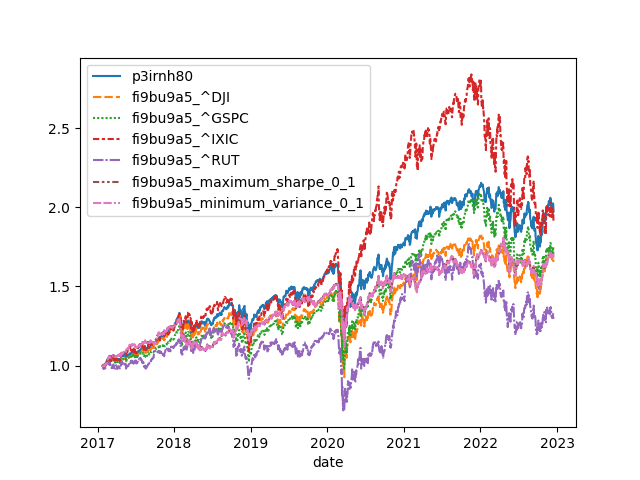
\includegraphics[width=\linewidth]{image/figure/returns_max}
            \caption{The model with Best Total Reward}
            \label{fig:returns_max}
        \end{subfigure}
        \hfill
        \begin{subfigure}{\experimentimgwidth\textwidth}
            \centering
            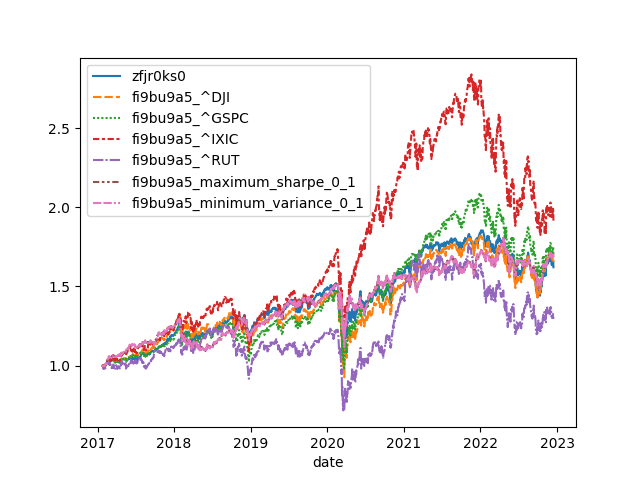
\includegraphics[width=\linewidth]{image/figure/returns_min}
            \caption{The model with The Smallest Cumulative Reward}
            \label{fig:returns_min}
        \end{subfigure}
        \caption{Cumulative return.}
        \label{fig:Cumulative Return}
    \end{figure}

    The image~\cref{fig:Cumulative Return} illustrates that a model can produce good results if it is configured with appropriate hyperparameters. Conversely, a model that is not configured with suitable hyperparameters fails to generate satisfactory results. The model that performs the best with optimal hyperparameters surpasses standard indexes such as S\&P 500 and DJIA, whereas the model that performs the worst with inadequate hyperparameters cannot outperform these benchmarks. How we tune hyperparameters is described in~\cref{subsec:hyperparameters}

    \begin{figure}[h!]
        \centering
        \begin{subfigure}[t]{0.3\textwidth}
            \centering
            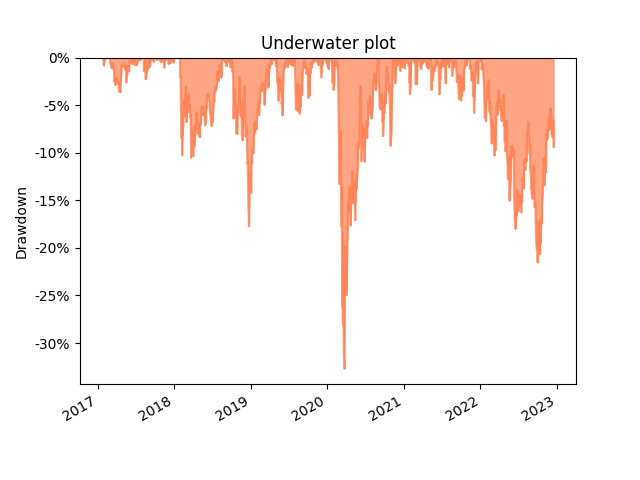
\includegraphics[width=\linewidth]{image/figure/drawdown_underwater_max}
            \caption{The model with The Highest Cumulative Reward}
            \label{fig:drawdown_underwater_max}
        \end{subfigure}
        \hfill
        \begin{subfigure}[t]{0.3\textwidth}
            \centering
            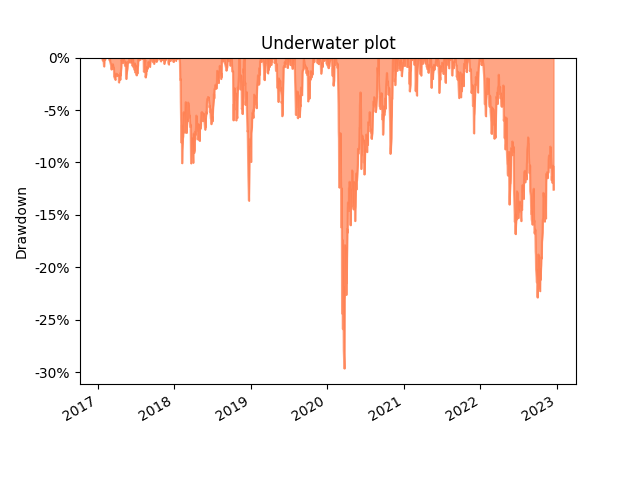
\includegraphics[width=\linewidth]{image/figure/drawdown_underwater_min}
            \caption{The model with The Smallest Cumulative Reward}
            \label{fig:drawdown_underwater_min}
        \end{subfigure}
        \hfill
        \begin{subfigure}[t]{0.3\textwidth}
            \centering
            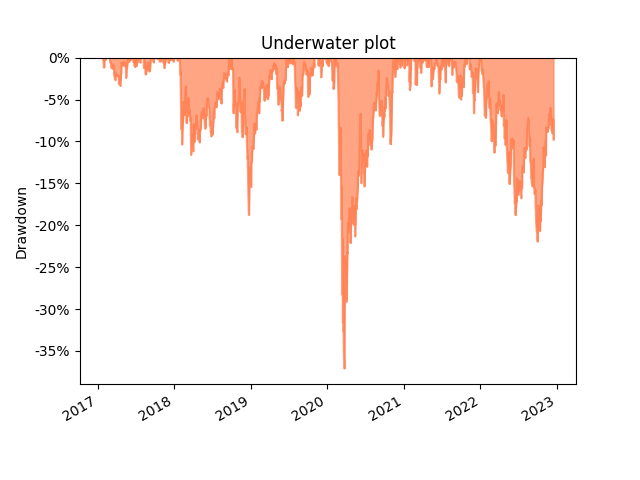
\includegraphics[width=\linewidth]{image/figure/drawdown_underwater_dji}
            \caption{The DJI index}
            \label{fig:drawdown_underwater_dji}
        \end{subfigure}
        \caption{The drawdowns.}
        \label{fig:Drawdown underwater}
    \end{figure}

    If we look at the drawdown graphs, they are literally the same, but ~\cref{fig:drawdown_underwater_max} is a bit worse than ~\cref{fig:drawdown_underwater_min} at large drawdowns. But~\cref{fig:drawdown_underwater_dji} is the worst of all at large drawdowns.

    \begin{figure}[h!]
        \centering
        \begin{subfigure}[b]{\experimentimgwidth\textwidth}
            \centering
            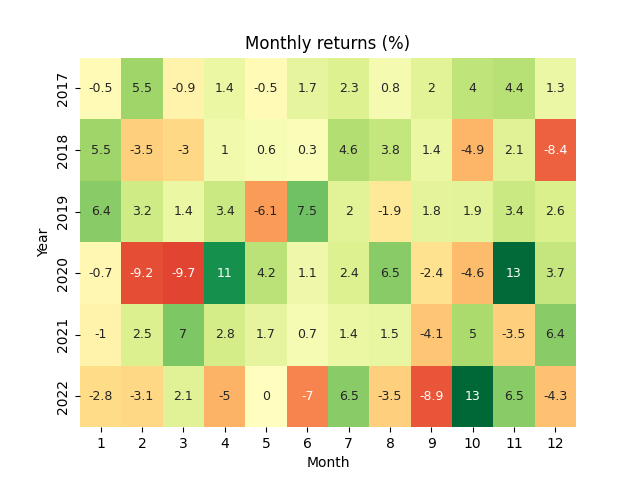
\includegraphics[width=\linewidth]{image/figure/monthly_returns_heatmap_max}
            \caption{The model with the highest cumulative reward}
        \end{subfigure}
        \hfill
        \begin{subfigure}{\experimentimgwidth\textwidth}
            \centering
            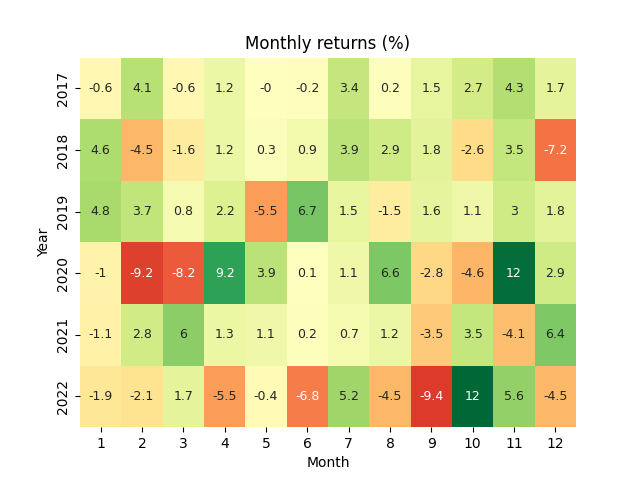
\includegraphics[width=\linewidth]{image/figure/monthly_returns_heatmap_min}
            \caption{The model with the smallest cumulative reward}
        \end{subfigure}
        \caption{The monthly returns.}
        \label{fig:Monthly returns heatmap}
    \end{figure}



    \begin{figure}[h!]
        \centering
        \begin{subfigure}[b]{\experimentimgwidth\textwidth}
            \centering
            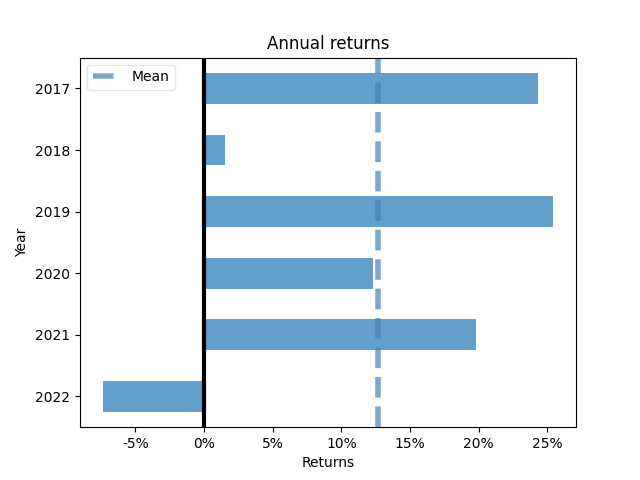
\includegraphics[width=\linewidth]{image/figure/annual_returns_max}
            \caption{The model with the highest cumulative reward}
        \end{subfigure}
        \hfill
        \begin{subfigure}{\experimentimgwidth\textwidth}
            \centering
            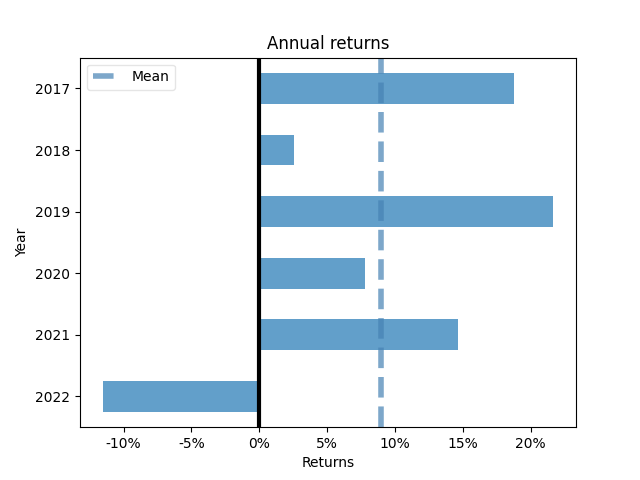
\includegraphics[width=\linewidth]{image/figure/annual_returns_min}
            \caption{The model with the smallest cumulative reward}
        \end{subfigure}
        \caption{The annual returns.}
        \label{fig:Annual returns}
    \end{figure}

    \begin{figure}[h!]
        \centering
        \begin{subfigure}[b]{\experimentimgwidth\textwidth}
            \centering
            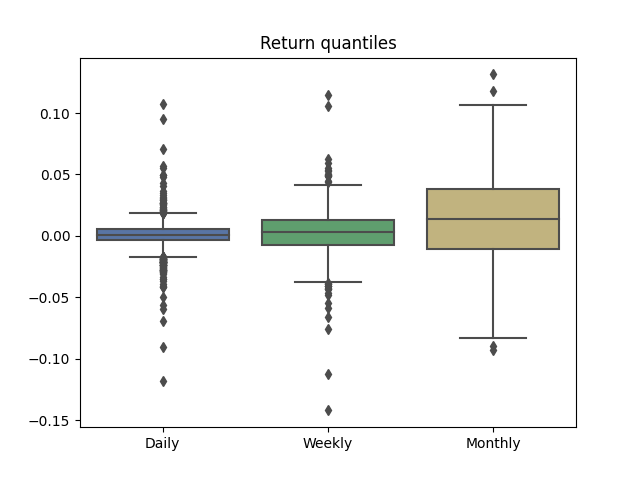
\includegraphics[width=\linewidth]{image/figure/return_quantiles_max}
            \caption{The model with the highest cumulative reward}
        \end{subfigure}
        \hfill
        \begin{subfigure}{\experimentimgwidth\textwidth}
            \centering
            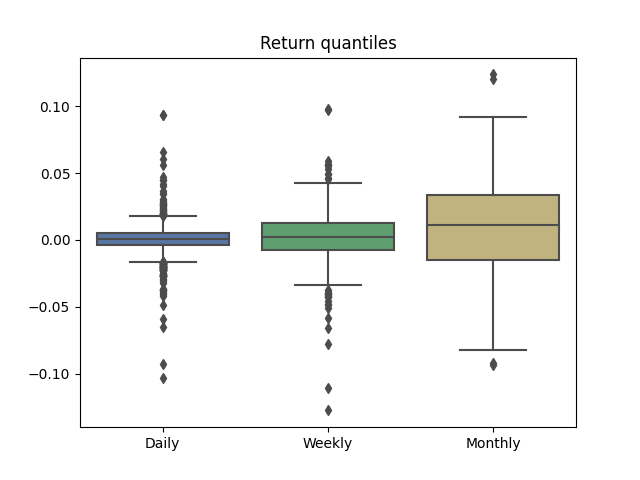
\includegraphics[width=\linewidth]{image/figure/return_quantiles_min}
            \caption{The model with the smallest cumulative reward}
        \end{subfigure}
        \caption{The quantiles of the returns.}
        \label{fig:Return quantiles}
    \end{figure}


    \begin{figure}[h!]
        \centering
        \begin{subfigure}[b]{\experimentimgwidth\textwidth}
            \centering
            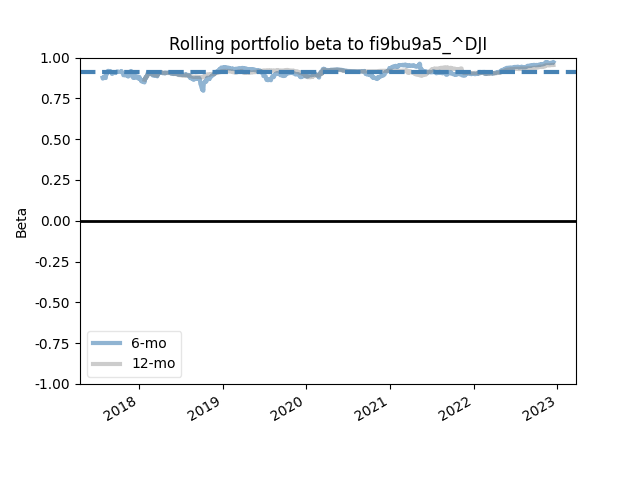
\includegraphics[width=\linewidth]{image/figure/rolling_beta_max}
            \caption{The model with the highest cumulative reward}
        \end{subfigure}
        \hfill
        \begin{subfigure}{\experimentimgwidth\textwidth}
            \centering
            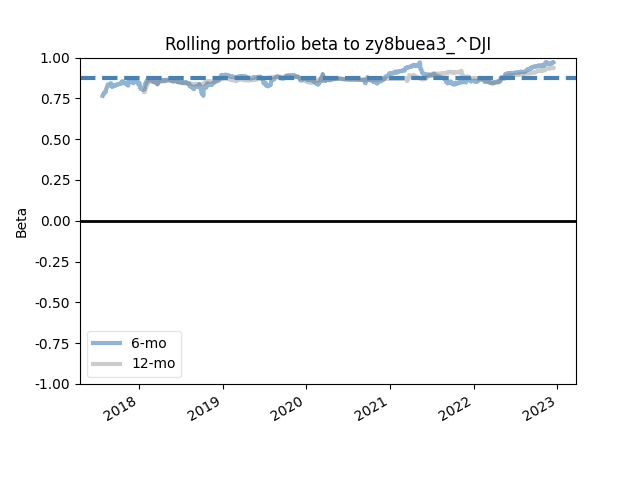
\includegraphics[width=\linewidth]{image/figure/rolling_beta_min}
            \caption{The model with the smallest cumulative reward}
        \end{subfigure}
        \caption{The rolling beta.}
        \label{fig:Rolling Beta}
    \end{figure}

%    \begin{figure}[h!]
%        \centering
%        \begin{subfigure}[b]{\experimentimgwidth\textwidth}
%            \centering
%            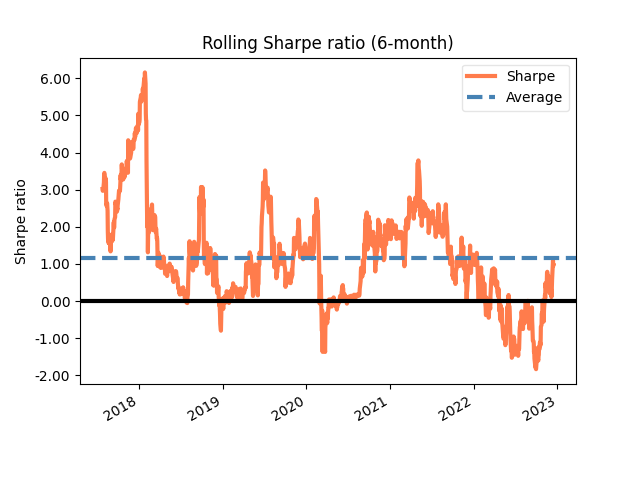
\includegraphics[width=\linewidth]{image/figure/rolling_sharpe_max}
%            \caption{The model with the highest cumulative reward}
%        \end{subfigure}
%        \hfill
%        \begin{subfigure}{\experimentimgwidth\textwidth}
%            \centering
%            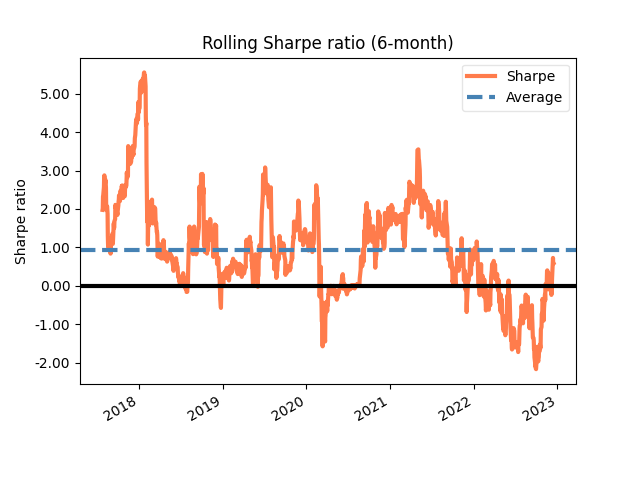
\includegraphics[width=\linewidth]{image/figure/rolling_sharpe_min}
%            \caption{The model with the smallest cumulative reward}
%        \end{subfigure}
%        \caption{The rolling Sharpe ratio.}
%        \label{fig:Rolling Sharpe}
%    \end{figure}

    \subsection{Reinforcement Learning Algorithms}\label{subsec:rl-algorithms}
    TODO

    \subsection{Hyperparameters}\label{subsec:hyperparameters}
    TODO


    \section{Summary}\label{sec:summary}
    TODO


\end{document}
